 % !TEX root = report.tex
 % !TEX program = xelatex
 
 键盘控制器模块负责接收PS/2接口传来的数据,并将按键最终转换为\texttt{VT220}规范中指定的指令序列从串口发送给PC。
 本模块主要由下列的子模块构成。

 \subsection{PS2接收模块 \texttt{Ps2Receiver}}

 本模块采样由PS/2接口发送来的键盘时钟与数据信号,在每次正确收到一个扫描码(8位二进制)后发出指示。
 由于键盘时钟远远慢于该模块运行的时钟频率,所以我们对键盘数据进行了8倍过采样,以最大程度地消除毛刺,保证数据的正确性。

 \subsection{扫描码译码模块 \texttt{ScancodeDecoder}}
 
 本模块用于将扫描码转换为控制命令序列。我们需要区分的情况有:
 \begin{description}
    \item[是否为特殊扫描码] 特殊扫描码以\texttt{E0}为前缀,此时的扫描码有至少2字节长。
    其中比较有代表性的一部分可见表\ref{tab:scancode_to_text}所示。其中\texttt{ESC}表示\texttt{0x1Bh}。
    较完整的内容可参见 \url{https://docs.microsoft.com/en-us/windows/console/console-virtual-terminal-sequences}。

    \begin{table}[htbp]
        \centering
        \caption{一些特殊按键扫描码与Escape Sequence对应关系}
        \label{tab:scancode_to_text}
        \begin{tabular}{|l|l|l|}
        \hline
        \textbf{Key}   & \textbf{Scancode} & \textbf{Escape Sequence}   \\ \hline
        Insert         & \texttt{E0 70}    & \texttt{ESC {[} 2 $\sim$}  \\ \hline
        Delete         & \texttt{E0 71}    & \texttt{ESC {[} 3 $\sim$}  \\ \hline
        Left Arrow     & \texttt{E0 6B}    & \texttt{ESC {[} D       }  \\ \hline
        Home           & \texttt{E0 6C}    & \texttt{ESC {[} H       }  \\ \hline
        End            & \texttt{E0 69}    & \texttt{ESC {[} F       }  \\ \hline
        Up Arrow       & \texttt{E0 75}    & \texttt{ESC {[} A       }  \\ \hline
        Down Arrow     & \texttt{E0 72}    & \texttt{ESC {[} B       }  \\ \hline
        Page Up        & \texttt{E0 7D}    & \texttt{ESC {[} 5 $\sim$}  \\ \hline
        Page Down      & \texttt{E0 7A}    & \texttt{ESC {[} 6 $\sim$}  \\ \hline
        Right Arrow    & \texttt{E0 74}    & \texttt{ESC {[} C       }  \\ \hline
        \end{tabular}
    \end{table}

    非特殊扫描码的按键中也有部分会产生较长的Escape Sequence,如\texttt{F1}到\texttt{F10}的功能键。为了节省篇幅,此处不再叙述。

    \item[是否按下Shift键] 这部分的处理比较简单,这是由于\texttt{VT220}规范中不包含使用Shift的组合键,故只要正常处理Shift的功能(即输出大写字母/键帽上靠上的字符)即可。

    \item[是否按下Ctrl键] 在 \texttt{VT220} 规范中,对于同时按下Ctrl与字母键发送的序列有详细的规定,可见 \url{https://vt100.net/docs/vt100-ug/table3-5.html}。
    需要特别处理的是Ctrl与特殊扫描码按键同时按下的情况,具体如表\ref{tab:ctrl_scancode}所示。

    \begin{table}[htbp]
        \centering
        \caption{Ctrl与特殊扫描码按键对应的Escape Sequence}
        \label{tab:ctrl_scancode}
        \begin{tabular}{|l|l|}
        \hline
        \textbf{Key}           & \textbf{Escape Sequence}  \\ \hline
        Ctrl + Up Arrow        & \texttt{ESC {[} 1 ; 5 A}  \\ \hline
        Ctrl + Down Arrow      & \texttt{ESC {[} 1 ; 5 B}  \\ \hline
        Ctrl + Right Arrow     & \texttt{ESC {[} 1 ; 5 C}  \\ \hline
        Ctrl + Left Arror      & \texttt{ESC {[} 1 ; 5 D}  \\ \hline
        \end{tabular}
    \end{table}
 \end{description}

 \subsection{PS2转换模块 \texttt{Ps2Translator}}
 本模块负责接收扫描码,并将每一个键盘事件(如按下一个按键或一个组合键)对应的Escape Sequence送入FIFO中待发送。
 本模块由一个较复杂的状态机实现,如图\ref{fig:ps2_translator}所示。

 \begin{figure}[htbp]
    \centering
    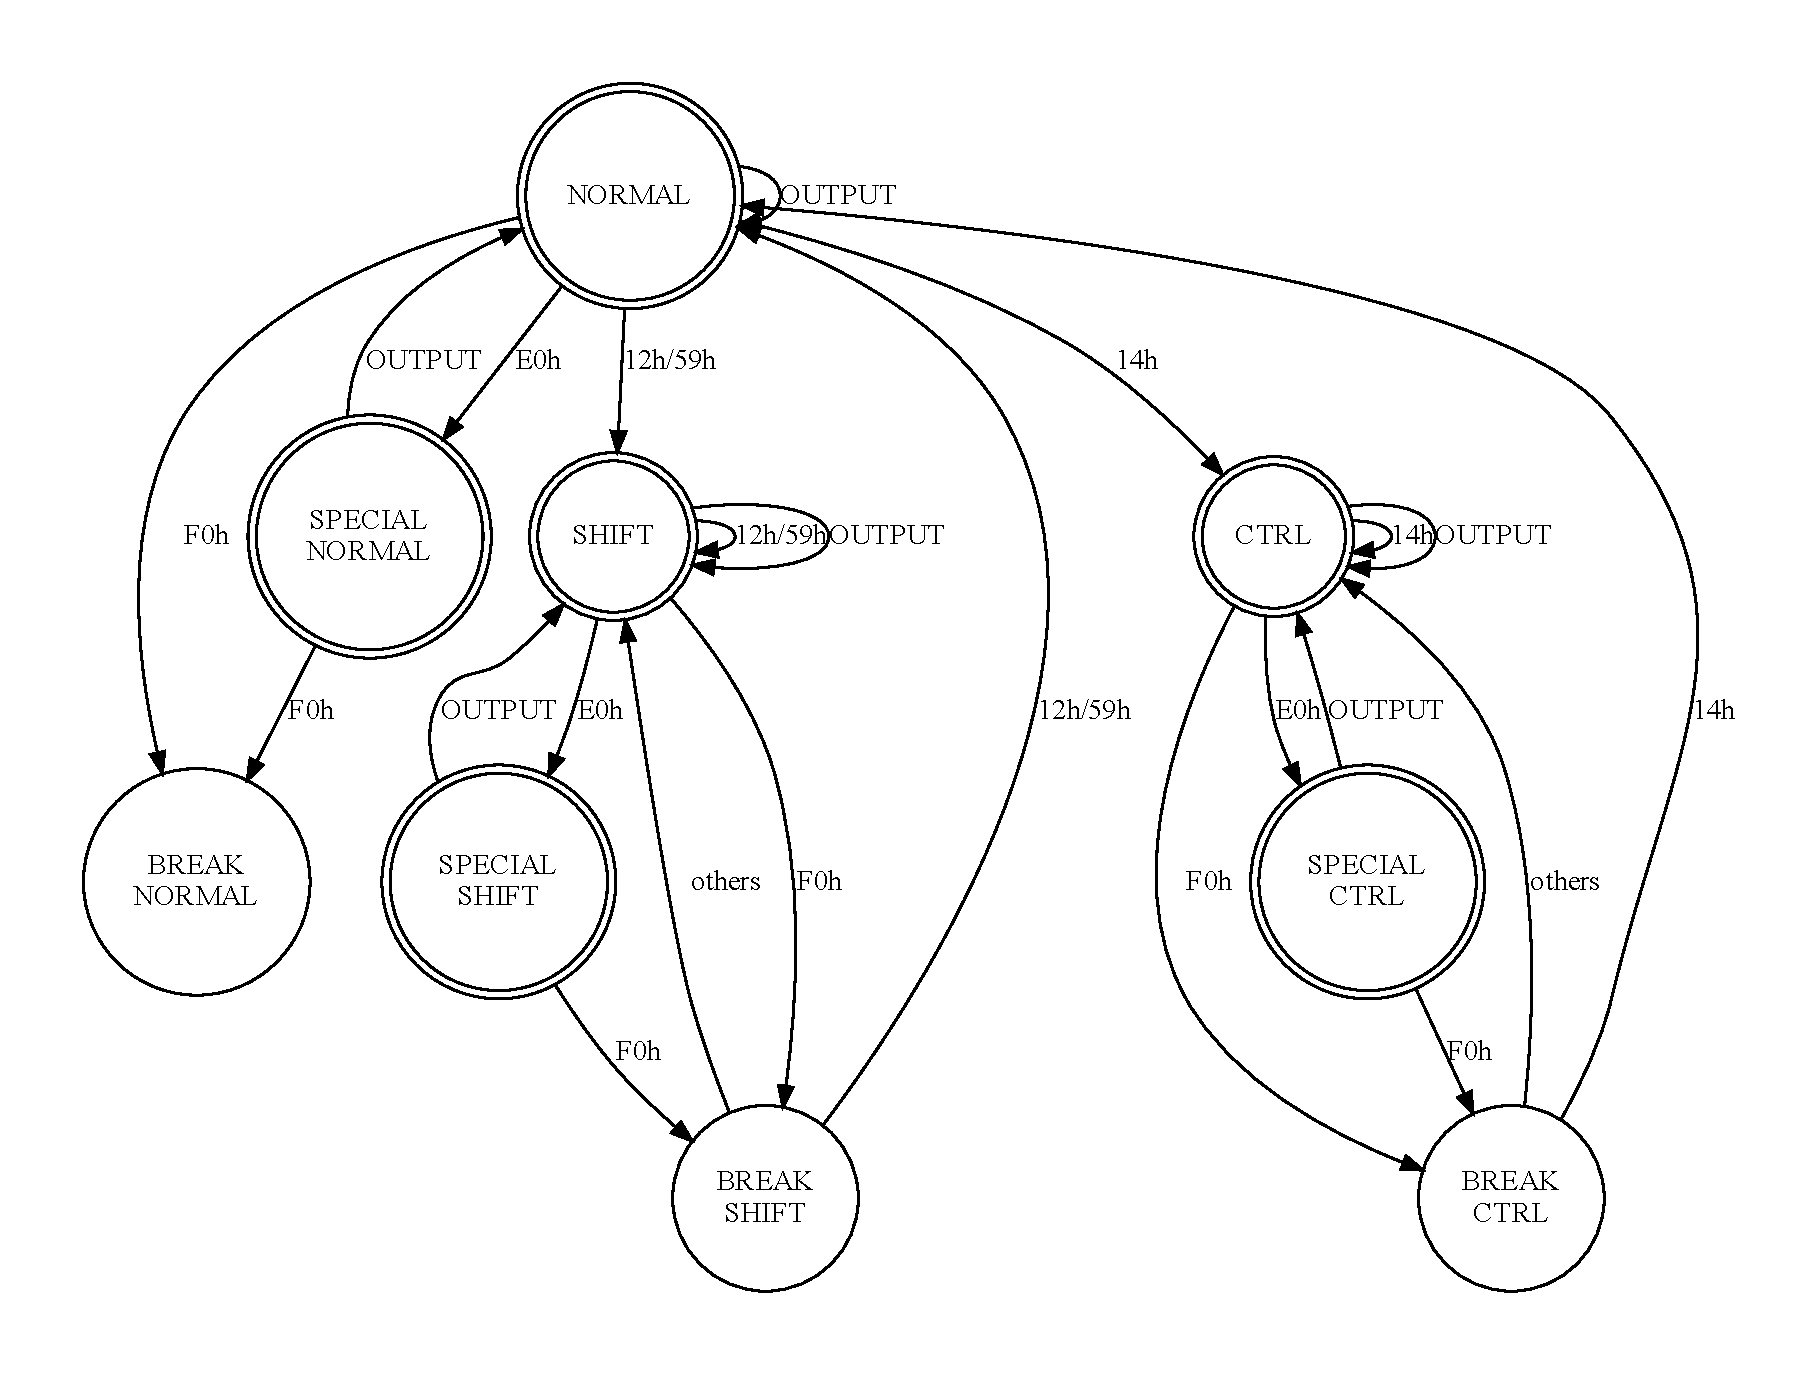
\includegraphics[width=\linewidth]{ps2_translator.pdf}
    \caption{PS2转换模块状态转移示意图}
    \label{fig:ps2_translator}
\end{figure}

其中转移边即为收到的扫描码,\texttt{OUTPUT}表示将此时收到的扫描码传给译码模块,并将得到的Escape Sequence推入FIFO中。
所有双圆圈标记的状态为可能产生输出的状态。

此模块可以正确地处理重复按键、多个按键等常见情况。当得到的按键或组合没有在\texttt{VT220}规范中时,本模块不会产生任何输出。

\subsection{FIFO数据格式}
PS2转换模块与串口发送模块之间通过一个FIFO进行数据缓冲。由于每个Escape Sequence序列的长度不会超过56字节,FIFO的位宽定为64比特,其中存储的数据格式如表\ref{tab:fifo_bytefield}所示。

\begin{table}[htbp]
   \centering
       \caption{FIFO中每条数据的格式}
       \label{tab:fifo_bytefield}
       \vspace{1em}
       \begin{bytefield}[bitwidth=0.5em,endianness=big,boxformatting={\centering\tt}]{64}
           \bitheader{0,8,16,24,32,40,48,56,64} \\
           \bitbox{8}{Length} & \bitbox{8}{Char 7} &
           \bitbox{8}{Char 6} & \bitbox{8}{Char 5} &
           \bitbox{8}{Char 4} & \bitbox{8}{Char 3} &
           \bitbox{8}{Char 2} & \bitbox{8}{Char 1} &
       \end{bytefield}
   \end{table}

\subsection{FIFO处理模块 \texttt{FifoConsumer}}
此模块的功能比较比较简单,由于串口的发送比较慢,故使用该模块配合FIFO进行缓冲。
此模块包含一个状态机,设计思路如下:

\begin{enumerate}
    \item 等待,直到FIFO不为空
    \item 从FIFO中读取一条数据(格式如表\ref{tab:fifo_bytefield}),根据长度跳到第一个待发送字符之前
    \item 读取一个字符,向串口送出,等待直到串口发送完成
    \item 如果还有字符没有发送完成,跳到3,否则跳到1
\end{enumerate}

事实上,由于要发送的数据总长度较短,我们直接使用状态名而不是一个变量来记录当前剩余的字符数量,根据\texttt{Length}属性跳转到相应状态。
这样实现的好处是节省了不必要的时钟周期,减少了逻辑单元的复杂度,但是导致状态数量增长到31个。
由于这些状态都可分为几个大类(读取、等待、跳转),代码比较类似,借助于\texttt{SystemVerilog}的\texttt{define}关键词与宏展开,实现一个这样一个看似复杂的状态机是很简洁的。